\section{Analytical Solutions}\label{Analytical_Solutions}\thispagestyle{SectionFirstPage} % Hide headers on the first page of the section
\lhead{Analytical Solutions}
\hspace{\parindent} In this chapter we will analytically solve the standard SIR model with the help of the paper by Tiberiu Harko et al. \cite{Tiberiu_Harko}.
Our goal at first is to get a second degree differential equation that is equivalent to the given system of differential equation,
with changed variables for a better readability.

\begin{subequations}\label{eq:SIR}
	\begin{empheq}[left=\empheqlbrace]{align}
		&x^{\prime} = -\beta x  y \label{eq:onea}
		\\
		&y^{\prime} = \beta x  y - \gamma y \label{eq:oneb}
		\\
		&z^{\prime} = \gamma z \label{eq:onec}
		\\
		&x + y + z = N
		\\
		&x_0 = N_1, y_0 = N_2, z_0 = N_3
	\end{empheq}
\end{subequations}
We begin by differentiating (\ref{eq:onea}) with respect to time t, and substituting y with $y = \frac{-x^{\prime}}{\beta x}$ from the same equation

\begin{equation} \label{eq:two}
	\begin{split}
		x^{\prime\prime} = -\beta(x^{\prime} y + x y^{\prime}) =
		-\beta\left( x^{\prime}\left(\frac{-x^{\prime}}{\beta x}\right) + x y^{\prime}\right)
		 & \implies \frac{-x^{\prime\prime}}{\beta} = \frac{-(x^{\prime})^{2}}{\beta x} + x y^{\prime}                             \\
		 & \implies x y^{\prime} = \frac{-x^{\prime\prime}}{\beta} + \frac{-(x^{\prime})^{2}}{\beta x}                             \\
		 & \implies y^{\prime} =  \frac{-1}{\beta}\left(\frac{-x^{\prime\prime}}{x} - \left(\frac{x^{\prime}}{x}\right)^{2}\right)
	\end{split}
\end{equation}
Next we insert $y = \frac{-x^{\prime}}{\beta x}$ from (\ref{eq:onea}) into (\ref{eq:oneb}) and equate it to (\ref{eq:two})

\begin{equation} \label{eq:three}
	\begin{split}
		-x^{\prime} + \frac{\gamma x^{\prime}}{\beta x} =
		\frac{-1}{\beta}\left(\frac{-x^{\prime\prime}}{x} - \left(\frac{x^{\prime}}{x}\right)^{2}\right)
		 & \implies \beta x^{\prime} - \frac{\gamma x^{\prime}}{x} = \frac{x^{\prime\prime}}{x} - \left(\frac{x^{\prime}}{x}\right)^{2}    \\
		 & \implies \frac{x^{\prime\prime}}{x} - \left(\frac{x^{\prime}}{x}\right)^{2} + \frac{\gamma x^{\prime}}{x} - \beta x^{\prime}= 0
	\end{split}
\end{equation}
We also have that from (\ref{eq:onea})  $y = \frac{-x^{\prime}}{\beta x}$ and from (\ref{eq:onec})  $y = \frac{z^{\prime}}{\gamma}$.
Equating them we get

\begin{equation} \label{eq:four}
	\frac{-x^{\prime}}{\beta x} = \frac{z^{\prime}}{\gamma}
	\implies z^{\prime} = -\frac{\gamma}{\beta}\left(\frac{x^{\prime}}{x}\right)
\end{equation}
\newpage Next we integrate (\ref{eq:four}) 


\begin{equation} \label{eq:five}
	\begin{split}
		c_{1} + z = -\frac{\gamma}{\beta} \int \frac{x^{\prime}}{x} \,dt
		 & \implies c_{1} + z = -\frac{\gamma}{\beta}\left(\ln(x) + c_{2}\right)                                       \\
		 & \implies \ln(x) = -\frac{\beta c_{1}}{\gamma} -\frac{\beta z}{\gamma} - c_{2}                               \\
		 & \implies x = e^{-\frac{\beta z}{\gamma}} \cdot e^{-\frac{\beta c_{1}}{\gamma} - c_{2}}                      \\
		 & \implies x = x_{0}e^{-\frac{\beta z}{\gamma}}  \hspace{\parindent}  \textrm{Where } x_{0} \textrm{ is an integration constant}
	\end{split}
\end{equation}
From (\ref{eq:five}) we get the relation

\begin{equation} \label{eq:six}
	x^{\prime} = -\frac{x_{0}\beta}{\gamma} z^{\prime} e^{-\frac{\beta z}{\gamma}}
\end{equation}
Now if we differentiate (\ref{eq:four}) and preform some manipulation we get

\begin{equation} \label{eq:seven}
	z^{\prime\prime} = -\frac{\gamma}{\beta}\left(\frac{x^{\prime\prime}}{x} - \left(\frac{x^{\prime}}{x}\right)^{2} \right)
\end{equation}
Finally if we combine (\ref{eq:six}), (\ref{eq:seven}) and (\ref{eq:four}) into (\ref{eq:three}) we get

\begin{equation} \label{eq:eight}
	z^{\prime\prime} = x_{0} \beta z^{\prime} e^{-\frac{\beta z}{\gamma}} - \gamma z^{\prime}
\end{equation}
Which is equivalent to the system of equation (\ref{eq:SIR}). \\
From this point we can solve the ODE by transforming (\ref{eq:eight}) into a Bernoulli type differential equation and solving it
by the given formula. Since this is out of scope for numerical methods class, the full solution can be found in appendix (\ref{appendix-b}).

\pagebreak

\begin{figure}[H]
	\caption{Graphical Examples of the Analytical Solution}
	\centering
	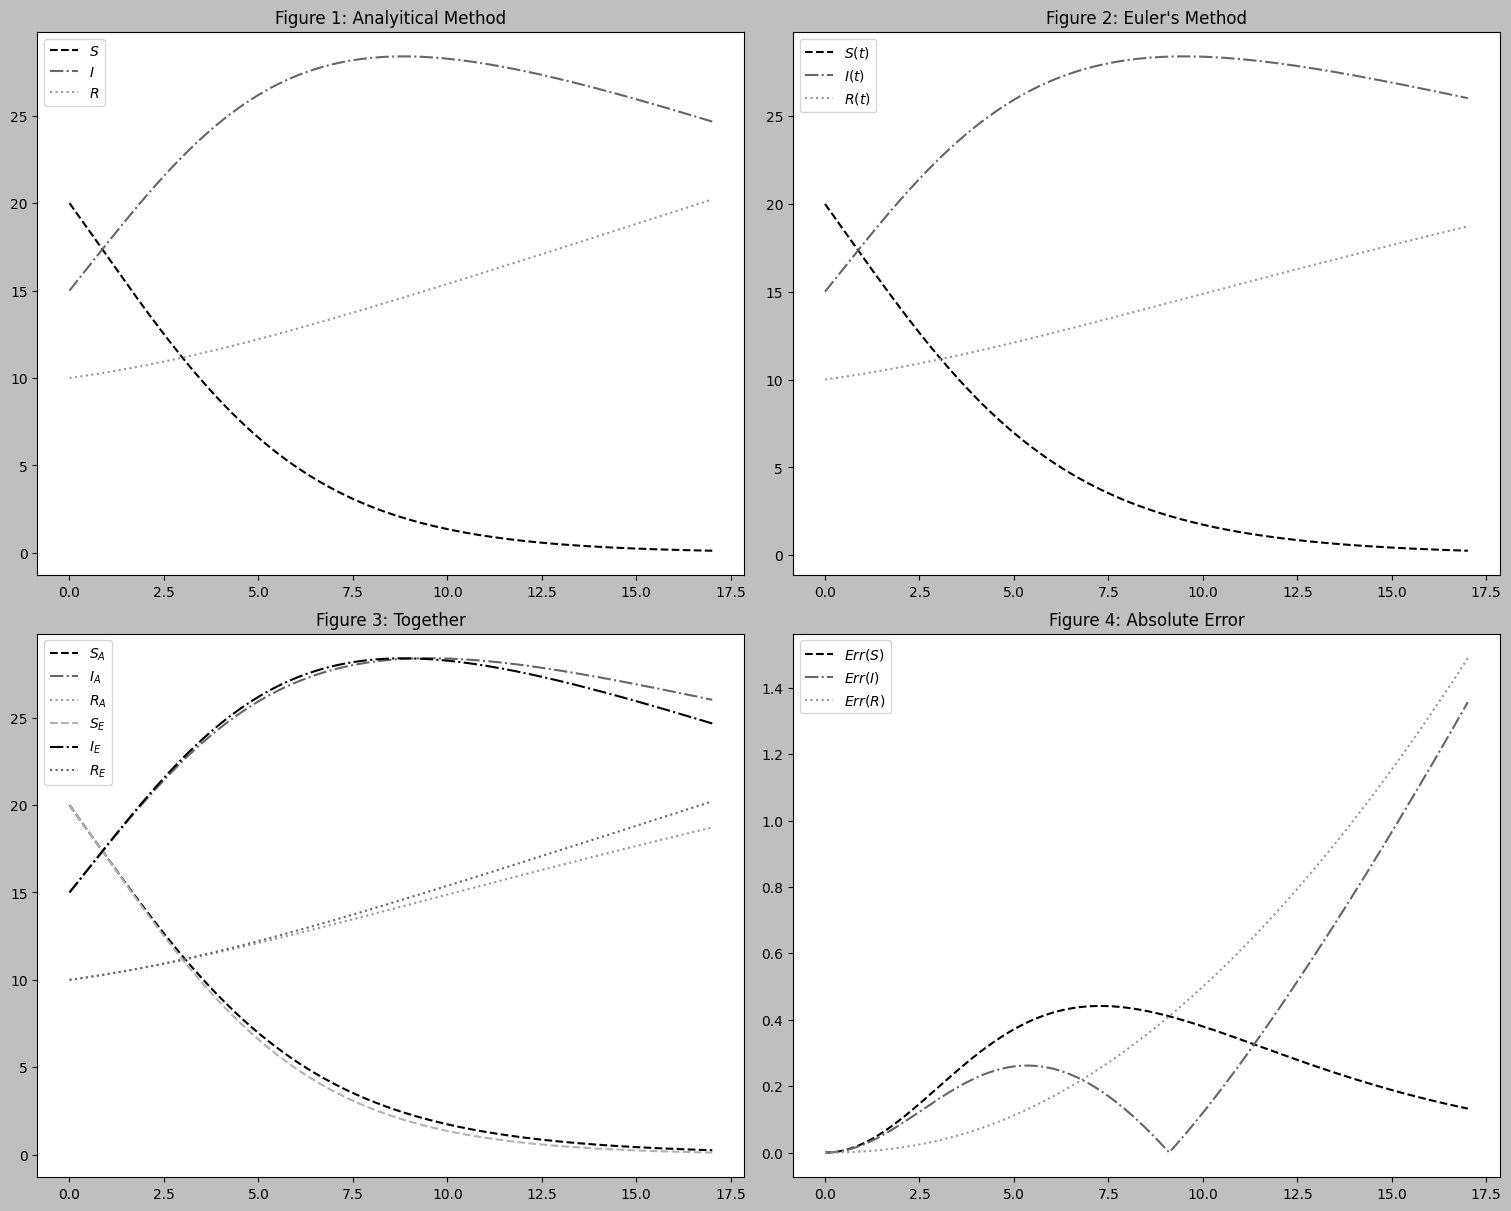
\includegraphics[width=16cm]{Figure_Analitical.png}
\end{figure}
Plotted Using Values$\quad$ $N_1=20, \quad N_2=15, \quad N_3=10, \quad \beta = 0.01, \quad \gamma = 0.02$

	

	

